%%%%%%%%%%%%%%%%%%%%%%%%%%%%%%%%%%%%%%%%%
% Beamer Presentation
% LaTeX Template
% Version 1.0 (10/11/12)
%
% This template has been downloaded from:
% http://www.LaTeXTemplates.com
%
% License:
% CC BY-NC-SA 3.0 (http://creativecommons.org/licenses/by-nc-sa/3.0/)
%
%%%%%%%%%%%%%%%%%%%%%%%%%%%%%%%%%%%%%%%%%

%----------------------------------------------------------------------------------------
%	PACKAGES AND THEMES
%----------------------------------------------------------------------------------------

\documentclass{beamer}

\newcommand{\EMSE}{ {\rm EMSE}}
\newcommand{\CC}{ {\rm CC}}
\newcommand{\MSE}{ {\rm MSE}}
\newcommand{\WIN}{\scriptscriptstyle {\rm WIE}}
\newcommand{\OROI}{\scriptscriptstyle {\rm out ROI}}
\newcommand{\Her}{\scriptscriptstyle H}
\newcommand{\T}{\scriptscriptstyle T}
\newcommand{\LMS}{\scriptscriptstyle {\rm LMS}}
\newcommand{\RDE}{\scriptscriptstyle {\rm RDE}}
\newcommand{\MRD}{\scriptscriptstyle {\rm MRD}}
\newcommand{\MSD}{\scriptscriptstyle {\rm MSD}}
\newcommand{\SBD}{\scriptscriptstyle {\rm SBD}}
\newcommand{\SDD}{\scriptscriptstyle {\rm SDD}}
\newcommand{\WIE}{\scriptscriptstyle {\rm WIE}}
\newcommand{\R}{\scriptscriptstyle {\rm R}}
\newcommand{\I}{\scriptscriptstyle {\rm I}}
\newcommand{\mT}{\scriptscriptstyle -T}
\newcommand{\vir}{,\hspace{-0.15ex}}
\newcommand{\M}{\scriptscriptstyle M}
\newcommand{\MMA}{\rm \scriptscriptstyle MMA}
\newcommand{\neigh}{\scriptscriptstyle {\rm neigh}}
\newcommand{\st}{\scriptscriptstyle {\rm st}}
\newcommand{\nd}{\scriptscriptstyle {\rm nd}}
\newcommand{\CSD}{\scriptscriptstyle {\rm CSD}}
\newcommand{\E}{{\rm E}}
\newcommand{\uM}{{\mathbf u}}
\newcommand{\rM}{{\mathbf r}}
\newcommand{\xM}{{\mathbf x}}
\newcommand{\yM}{{\mathbf y}}
\newcommand{\XM}{{\mathbf X}}
\newcommand{\w}{{\mathbf w}}
\newcommand{\wo}{{\mathbf{w}}_{\rm o}}
\newcommand{\q}{{\mathbf q}}
\newcommand{\qp}{{\mathbf {\dot{q}}}}
\newcommand{\Nuquad}{\|{\mathbf u(n)}\|^2}
\newcommand{\NuquadP}{\|{\mathbf u(n)}\|^2_{{\mathbf R}^{-1}(n)}}
\newcommand{\uMc}{{\mathbf u}^{\ast}}
\newcommand{\wtil}{\widetilde{\mathbf w}}
\newcommand{\Dw}{\boldsymbol{\Delta}{\mathbf w}}
\newcommand{\Dewp}{\boldsymbol{\Delta}{\mathbf{\dot{w}}}}
\newcommand{\Pb}{{\mathbf R}^{-1}}
\newcommand{\ebari}{{\bar{e}}_i}
\newcommand{\field}[1]{\mathbb{#1}}
\newcommand{\re}{\field{R}}
\newcommand{\co}{\field{C}}
\newcommand{\CO}{\field{C}}
\newcommand{\RE}{\field{R}}
\newcommand{\Tr}{{\rm Tr}}
\newcommand{\Ru}{{\mathbf R}}
\newcommand{\sgbeta}{\sigma_{\scriptscriptstyle{\!\alpha}}^2}
\newcommand{\sgphi}{\sigma_{\scriptscriptstyle{\!\varphi}}^2}
\newcommand{\cred}{\textcolor{red}}
\newcommand{\lbo}{\lambda_{\rm o}}
\newcommand{\cond}{\mathbf{w}_1(n\!-\!1),\mathbf{w}_{2}(n\!-\!1)}
\newcommand{\cb}{\textcolor{blue}}
\newcommand{\pu}{\mathbf{p}_{\!\scriptscriptstyle \Delta}}
\definecolor{laranja}{rgb}{0.8,0.5,0}
\newcommand{\crt}{\textcolor{laranja}}
\newcommand{\Psibf}{\boldsymbol{\Psi}}
\newcommand{\Sigmabf}{\boldsymbol{\Sigma}}
\newcommand{\epsbf}{\boldsymbol{\epsilon}}
\newcommand{\betabf}{\boldsymbol{\beta}}
\newcommand{\alphabf}{\boldsymbol{\alpha}}
\newcommand{\thetabf}{\boldsymbol{\theta}}
\newcommand{\gammabf}{\boldsymbol{\gamma}}
\newcommand{\lambdabf}{\boldsymbol{\lambda}}
\newcommand{\ML}{{\rm ML}}
\newcommand{\LS}{{\rm LS}}
\newcommand{\SSS}{{\rm SS}}
\newcommand{\UPS}{{\rm UPS}}
\newcommand{\PS}{{\rm PS}}

\mode<presentation> {

% The Beamer class comes with a number of default slide themes
% which change the colors and layouts of slides. Below this is a list
% of all the themes, uncomment each in turn to see what they look like.

%\usetheme{default}
%\usetheme{AnnArbor}
%\usetheme{Antibes}
%\usetheme{Bergen}
%\usetheme{Berkeley}
%\usetheme{Berlin}
%\usetheme{Boadilla}
\usetheme{CambridgeUS}
%\usetheme{Copenhagen}
%\usetheme{Darmstadt}
%\usetheme{Dresden}
%\usetheme{Frankfurt}
%\usetheme{Goettingen}
%\usetheme{Hannover}
%\usetheme{Ilmenau}
%\usetheme{JuanLesPins}
%\usetheme{Luebeck}
%\usetheme{Madrid}
%\usetheme{Malmoe}
%\usetheme{Marburg}
%\usetheme{Montpellier}
%\usetheme{PaloAlto}
%\usetheme{Pittsburgh}
%\usetheme{Rochester}
%\usetheme{Singapore}
%\usetheme{Szeged}
%\usetheme{Warsaw}

% As well as themes, the Beamer class has a number of color themes
% for any slide theme. Uncomment each of these in turn to see how it
% changes the colors of your current slide theme.

%\usecolortheme{albatross}
%\usecolortheme{beaver}
%\usecolortheme{beetle}
%\usecolortheme{crane}
%\usecolortheme{dolphin}
%\usecolortheme{dove}
%\usecolortheme{fly}
%\usecolortheme{lily}
%\usecolortheme{orchid}
%\usecolortheme{rose}
%\usecolortheme{seagull}
%\usecolortheme{seahorse}
%\usecolortheme{whale}
%\usecolortheme{wolverine}

%\setbeamertemplate{footline} % To remove the footer line in all slides uncomment this line
\setbeamertemplate{footline}[page number] % To replace the footer line in all slides with a simple slide count uncomment this line

\setbeamertemplate{navigation symbols}{} % To remove the navigation symbols from the bottom of all slides uncomment this line
}

\usepackage{graphicx} % Allows including images
\usepackage{booktabs} % Allows the use of \toprule, \midrule and \bottomrule in tables
\usepackage{color}
\usepackage{amsmath}
%----------------------------------------------------------------------------------------
%	TITLE PAGE
%----------------------------------------------------------------------------------------

\title[TopicModel]{Corpus preprocessing, cleaning and homogeneization with NLTK examples} % The short title appears at the bottom of every slide, the full title is only on the title page

\author{Jer\'onimo Arenas-Garc\'{\i}a, Vanessa G\'omez-Verdejo, Jes\'us Cid-Sueiro} % Your name
\institute[UC3M] % Your institution as it will appear on the bottom of every slide, may be shorthand to save space
{
Universidad Carlos III de Madrid \\ % Your institution for the title page
\medskip
\textit{jeronimo.arenas@uc3m.es} % Your email address
}
\date{March 16, 2021}
%\date{\today} % Date, can be changed to a custom date

\begin{document}

%######################################################
%######################################################
\begin{frame}
\titlepage % Print the title page as the first slide
\end{frame}


%######################################################
%######################################################
\section{Corpus preprocessing}


%######################################################
%######################################################
\begin{frame}

    \frametitle{Document representation for Machine Learning}

    \begin{itemize}
  
    	\item ML algorithms process numbers, not words
    	\item We need to transform text into meaningful numbers
    	\item Bag-of-Words (BoW) representation: Count number of appearances of each word (in the vocabulary of all documents) in a given document
    	\item In order to have a useful representation, some preprocessing steps are normally required
    
    \end{itemize}
    
    \vspace{1cm}
    
    \centerline{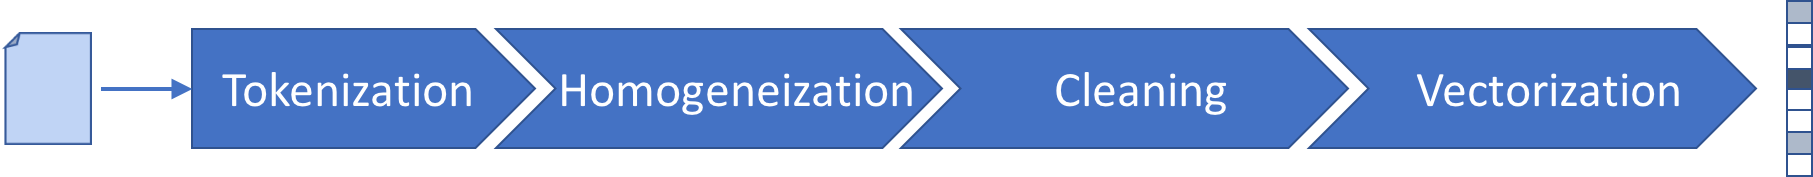
\includegraphics[width=\textwidth]{./figs/NLPTM_doc_preproc.png}}

\end{frame}


%######################################################
%######################################################
\subsection{Natural Language Processing Toolkit (NLTK)}

%######################################################
%######################################################
\begin{frame}

\frametitle{NLP with Python}

	\begin{columns}
	
	\begin{column}{.5\textwidth}
	
	NLTK:
	
	\small
		\begin{itemize}
			\item Basic classes for representing data relevant to NLP
			
			\item Functions for performing common NLP tasks
			
			\item Corpuses
			
		\end{itemize}
	
	\normalsize
	Spacy:
	
	\small
		\begin{itemize}
			
			\item NLP Pipelines ready for production
			
			\item Incorporates pre-trained Neural Networks Models
			
			\item It is possible to fine tune the models
			
		\end{itemize}

	\end{column}
	
	\begin{column}{.5\textwidth}
		\vspace{.2cm}			\centerline{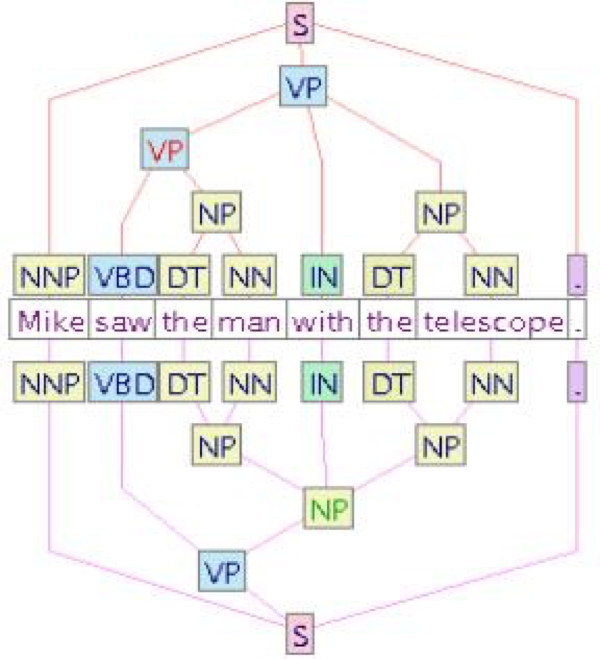
\includegraphics[width=\textwidth]{./figs/NLPTM_NLTKgeneral.png}}
	\end{column}

	\end{columns}
	

\end{frame}

%######################################################
%######################################################
\begin{frame}

\frametitle{NLTK modules}

	\begin{itemize}
			
		\item corpora: a package containing collections of example text 
		\item {\bf tokenize}: functions to split text strings into basic elements
		\item probability: for modeling frequency distributions and probabilistic systems 
		\item {\bf stem}:  package of functions to stem words of text 
		\item {\bf wordnet}: interface to the {\color{blue}{\href{https://wordnet.princeton.edu/}{WordNet}}} lexical resource 
		\item chunk: identify short non-nested phrases in text 
		\item {\bf tag}: tagging each word with part-of-speech, sense, etc. 
		\item parse: building trees over text - recursive descent, shift-reduce, probabilistic, etc. 
		\item cluster: clustering algorithms 
		\item draw: visualize NLP structures and processes 
		\item contrib: various pieces of software from outside contributors 

	\end{itemize}

\end{frame}


%######################################################
%######################################################
\subsection{Tokenization}

%######################################################
%######################################################
\begin{frame}

    \frametitle{Tokenization}

    \centerline{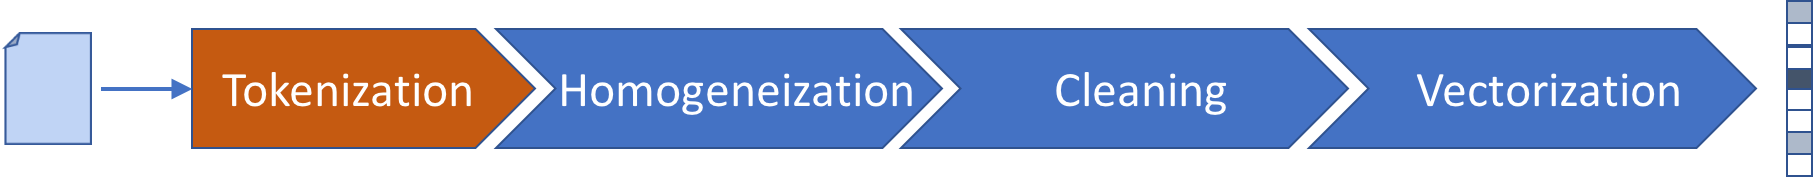
\includegraphics[width=\textwidth]{./figs/NLPTM_tokenization.png}}

    \begin{itemize}
  
    	\item The goal is to find the basic elements (tokens) of a given string. 
    	\item Python {\tt split()} function makes a list from a string using a given substring as a separator
    	\item NLTK tokenizers are better suited to this task, and more efficient since they use regular expressions.
    	\item Includes both sentence and word tokenizers
    	
    \end{itemize}
    
    \footnotesize
    \begin{block}{Example}
    	\begin{itemize}
    		\footnotesize
    		\item[] $\gg$ {\tt sentence = 'Hello, world.'}
    		\item[] $\gg$ {\tt sentence.split()}
    		\item[] {\tt ['Hello,', 'world.']}
    		\item[] $\gg$ {\tt from nltk.tokenize import word\_tokenize}
    		\item[] $\gg$ {\tt tokens = word\_tokenize(sentence)}
    		\item[] $\gg$ {\tt tokens = [el for el in tokens if el.isalnum()]}
    		\item[] {\tt ['Hello', 'world']}
    	
    	\end{itemize}
    \end{block}
    
\end{frame}


%######################################################
%######################################################
\subsection{Homogenization}

%######################################################
%######################################################
\begin{frame}

    \frametitle{Homogenization}

    \centerline{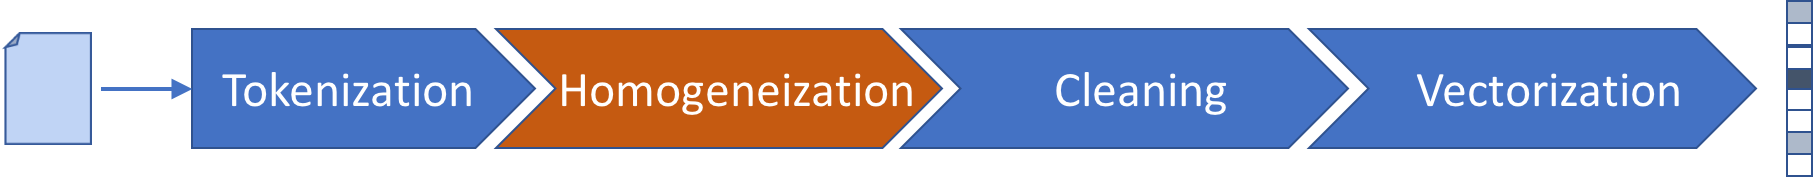
\includegraphics[width=\textwidth]{./figs/NLPTM_homogenization.png}}

    \begin{itemize}
    	\item Collapse semantically equivalent words into a unique representative
    		\begin{itemize}
    			\item Different forms of a word: \\ 
    			organize, organizes, organizing, ... $\rightarrow$ organize 
    			\item Derivationally related words with similar meanings: \\ democracy, democratic, democratization, ... $\rightarrow$ democracy
    		\end{itemize}
    		
    	\item Stemming vs lemmatization
    		\begin{itemize}
    			\item {\bf Stemming} chops of the ends of words using a list of suffixes
    			\item {\bf Lemmatization} usually refers to doing things properly with a vocabulary and morphological analysis of words, aiming to return the base or dictionary form (lemma) of a word. 
				\item A practical difference is that lemmatizers output complete words.

    		\end{itemize}
    		
    	%\item If using case sensitive implementations, we need to lowercase the tokens as a preliminary step
    	
    	\item An additional benefit is a smaller vocabulary size (vector length)
    	
    \end{itemize}
    
\end{frame}


%######################################################
%######################################################
\begin{frame}

    \frametitle{Stemming}
    
        \begin{block}{}
        \begin{itemize}
            \item Porter algorithm:  developed by Martin Porter in 1980. Not very aggressive
            \item Based on a set of expert rules. Ignores words roles
            \item NLTK incorporates SnowBallStemmer that fixes some issues of the Porter algorithm
            \item Output not necessarily `proper' words
        \end{itemize}
        \end{block}

        \footnotesize
        \begin{itemize}
    		\item[] $\gg$ {\tt import nltk.stem}
    		\item[] $\gg$ {\tt s = nltk.stem.SnowballStemmer('english')}
    		\item[] $\gg$ {\tt s.stem('image')} $\rightarrow$ {\tt 'imag'}
    		\item[] $\gg$ {\tt s.stem('images')} $\rightarrow$ {\tt 'imag'}
    		\item[] $\gg$ {\tt s.stem('organize')} $\rightarrow$ {\tt 'organ'}
    		\item[] $\gg$ {\tt s.stem('organizing')} $\rightarrow$ {\tt 'organ'}
			\item[] $\gg$ {\tt s.stem('organ')} $\rightarrow$ {\tt 'organ'}
    	\end{itemize}

\end{frame}


%######################################################
%######################################################
\begin{frame}

    \frametitle{Lemmatization}
    
    	\begin{block}{}
    	\begin{itemize}
    	\item NLTK recurs to WordNet, a lexical database for the English language. Wordnet groups English words into sets of synonyms called synsets.
    	\item With contextual information (the grammatical role of the word) {\tt lemmatize()} can filter grammatical differences
    	\end{itemize}
    	\end{block}
    	
    	\begin{itemize}
    		\footnotesize
    		\item[] $\gg$ {\tt from nltk.stem import WordNetLemmatizer}
    		\item[] $\gg$ {\tt wnl = WordNetLemmatizer()}
    		\item[] $\gg$ {\tt wnl.lemmatize('image')} $\rightarrow$ {\tt 'image'}
    		\item[] $\gg$ {\tt wnl.lemmatize('images')} $\rightarrow$ {\tt 'image'}
    		\item[] $\gg$ {\tt wnl.lemmatize('organize')} $\rightarrow$ {\tt 'organize'}
    		\item[] $\gg$ {\tt wnl.lemmatize('organizing')} $\rightarrow$ {\tt 'organizing'}
    		\item[] $\gg$ {\tt wnl.lemmatize('organizing', pos='v')} $\rightarrow$ {\tt 'organize'}
    		\item[] $\gg$ {\tt wnl.lemmatize('organ')} $\rightarrow$ {\tt 'organ'}
       	\end{itemize}
    
\end{frame}

%######################################################
%######################################################
\begin{frame}

\frametitle{NLP lemmatizers for Python}

\footnotesize
\begin{itemize}
    \item Different algorithm and performances
    \item Different computational requirements
\end{itemize}


\centerline{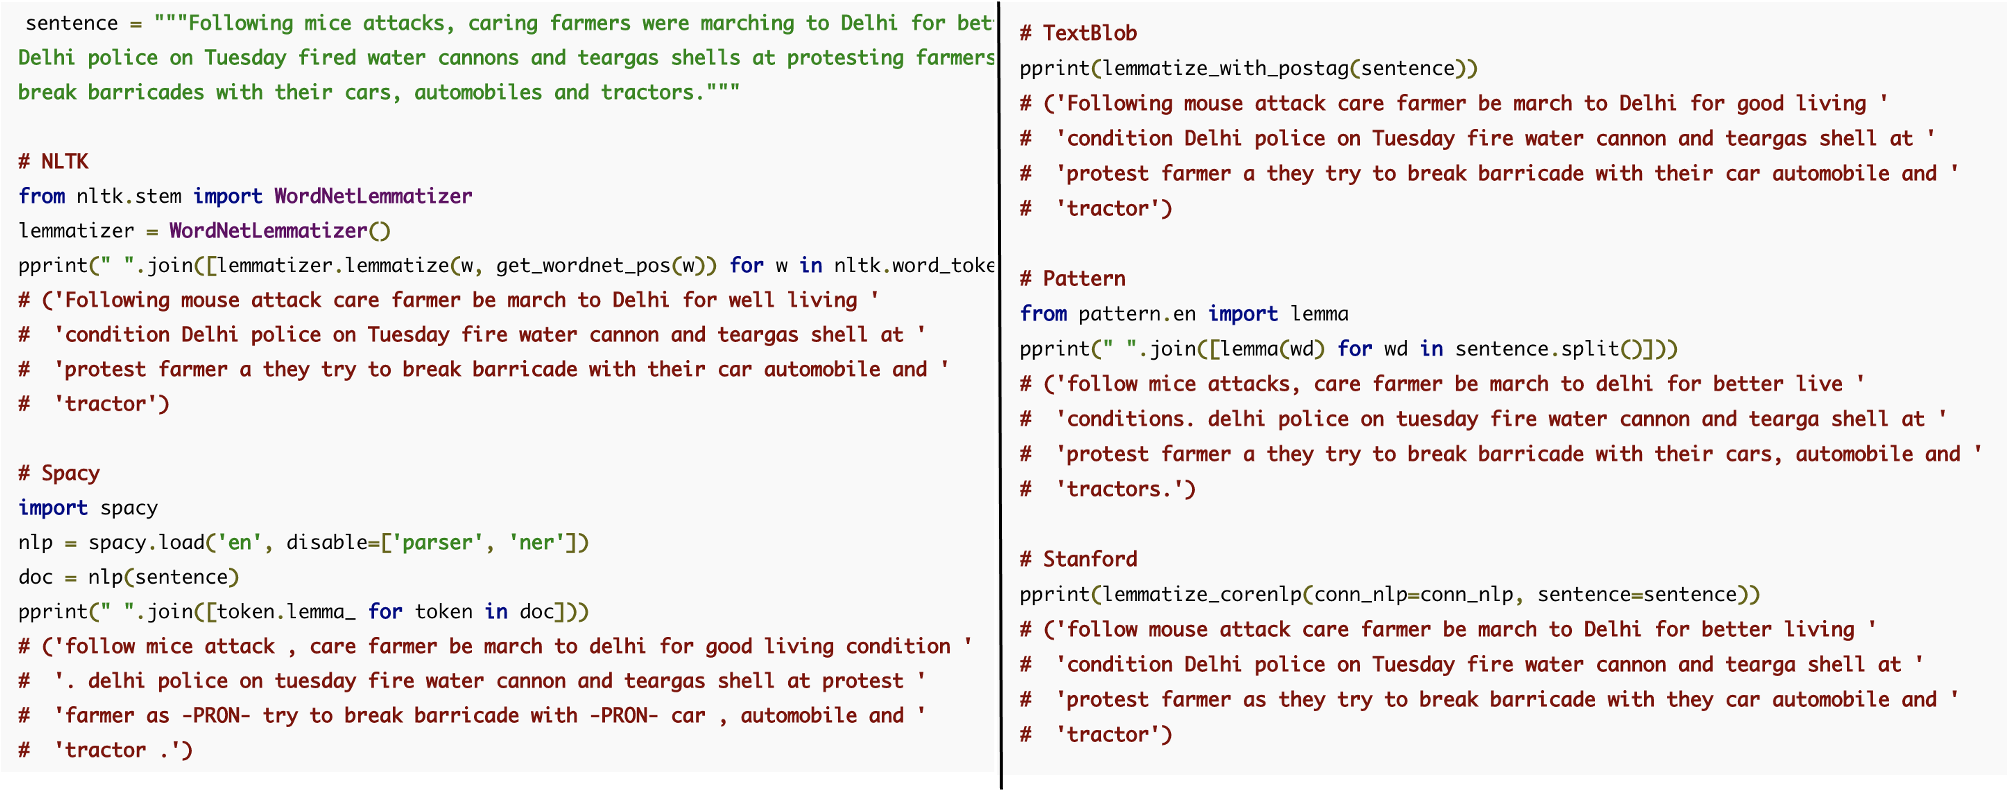
\includegraphics[width=\textwidth]{./figs/lemmas.png}}
\tiny
Taken from \url{https://www.machinelearningplus.com/nlp/lemmatization-examples-python/}
\end{frame}

%######################################################
%######################################################
\begin{frame}

    \frametitle{Other homogeneization tasks}
    
    	\begin{block}{Part of Speech Tagging}
    	\begin{itemize}
    	\item Part-of-speech (POS) tagging is the process of assigning a word to its grammatical category (noun, verb, adverb,…), in order to understand its role within the sentence.
    	\item POS tagging provides the contextual information to {\tt lemmatize()} to filter grammatical differences.

    	\end{itemize}
    	\end{block}
    	
    	\begin{itemize}
    		\footnotesize
    		\item[] $\gg$ {\tt from nltk import pos\_tag}
    		\item[] $\gg$ {\tt tokens = word\_tokenize('This is a simple sentence') }
    		\item[] $\gg$ {\tt pos\_tag(tokens)}
    		\item[] {\tt [('This', 'DT'), ('is', 'VBZ'), ('a', 'DT'), ('simple', 'JJ'), ('sentence', 'NN')]}
       	\end{itemize}
    
    	\begin{block}{N-gram detection}
        	\begin{itemize}
        	\item Identification of groups of words that occasionally appear together, and have an inherent semantic value
        	\item E.g.: Machine learning, big data, etc
        	\end{itemize}
        \end{block}
    
\end{frame}


%######################################################
%######################################################
\subsection{Cleaning}

%######################################################
%######################################################
\begin{frame}

    \frametitle{Cleaning}

    \centerline{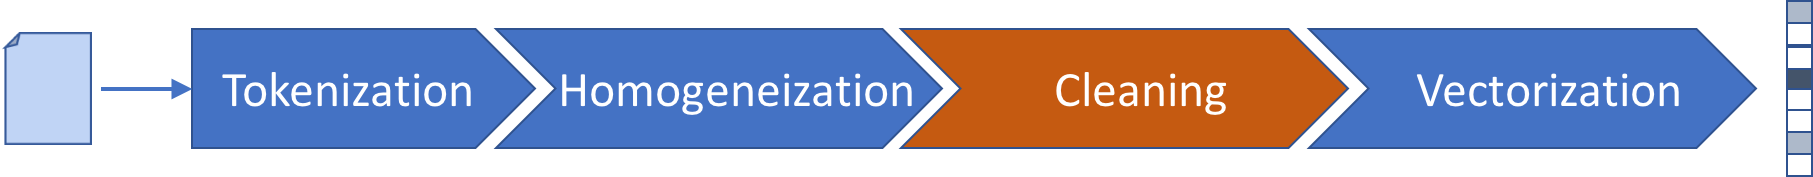
\includegraphics[width=\textwidth]{./figs/NLPTM_cleaning.png}}

\footnotesize

    \begin{block}{Stopword removal}
    		\begin{itemize}
    			\item Stopwords: Words that appear very often in all sorts of different contexts (language function words). They are removed by using stopwords lists
    			\item Very rare terms: Words that appear in a very reduced number of documents in the collection
    			\item Corpus specific stopwords: Words that are very common for a particular data set, or simply do not have significant semantic value for the application at hand. Either manually created lists, or by word frequency.
    		\end{itemize}
    \end{block}
    \begin{block}{Diccionary of equivalent terms}
        \begin{itemize}
        	\item Lists of words that should be considered equivalent for the document collection
        	\item Word replacement efficiently implemented using regular expressions \url{https://www.w3schools.com/python/python_regex.asp}
        \end{itemize}
    \end{block}			
    
\end{frame}


%######################################################
%######################################################
\subsection{Vectorization}

%######################################################
%######################################################
\begin{frame}

    \frametitle{Vectorization: Bag-of-words representation}

    \centerline{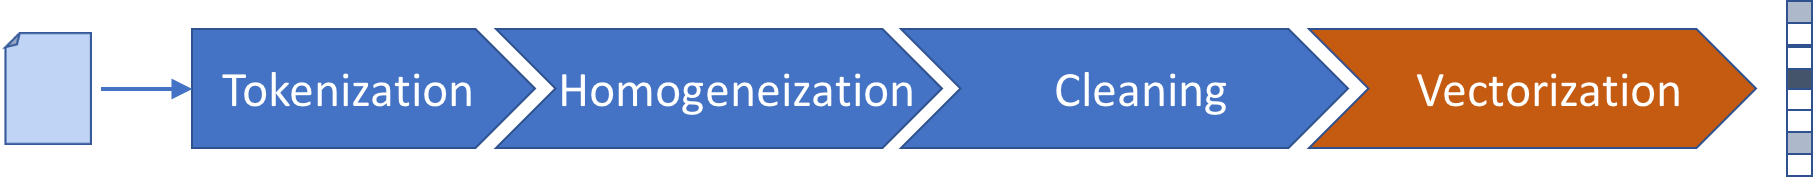
\includegraphics[width=\textwidth]{./figs/NLPTM_vectorization.png}}

    The goal is to convert the sequence of homogenized and cleaned tokens into a numeric vector
    \begin{itemize}
    	\item Bag-of-words representation: counts how many appearances of each word occur in each document
    	\item Each position in the vector is associated to a unique word in the vocabulary, so vectors are typically very sparse
    \end{itemize}
    
    \vspace{.2cm}
    \centerline{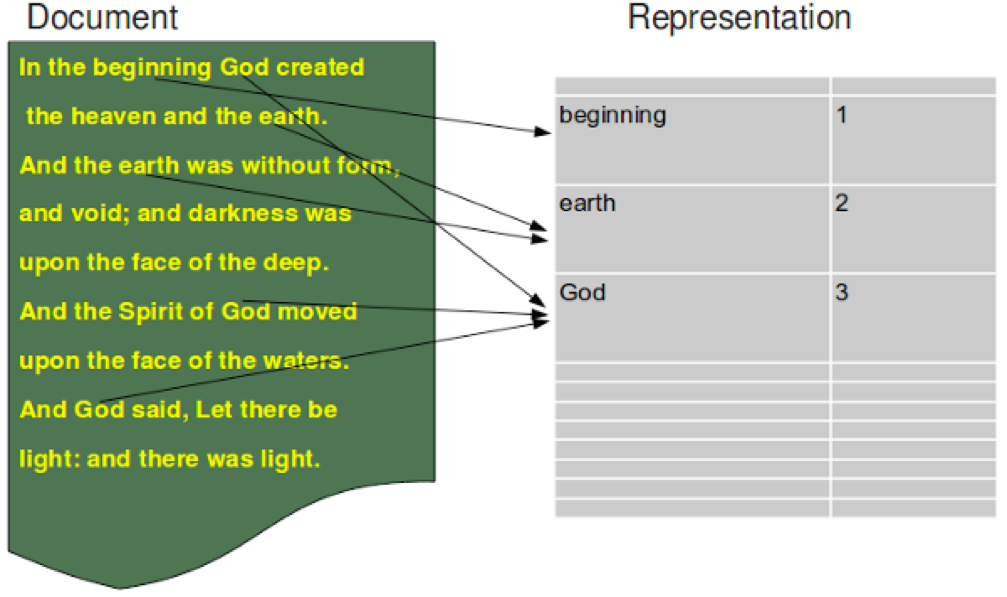
\includegraphics[width=.5\textwidth]{./figs/NLPTM_BoW.png}}
    			    
\end{frame}


%######################################################
%######################################################
\begin{frame}

    \frametitle{Term frequency - Inverse document frequency (TF-IDF)}

    We want a high value for a given term in a given doc if that term occurs often in that particular doc and very rarely anywhere else

\vspace{1cm}

	\begin{itemize}
	
	\item ${\rm TF}(w,d) = \frac{{\rm BoW}(w,d)}{\# {\text{ words in } d}}$
	\item ${\rm IDF}(w) = \log \frac{\# {\text{ docs}}}{\# {\text{ docs with term } w}}$
	\item ${\rm TF-IDF}(w,d) = {\rm TF}(w,d) \times {\rm IDF}(w)$
		
	\end{itemize}
	
\vspace{1cm}
	
	The IDF term emphasizes the words that appear in a reduced number of documents.
    			    
\end{frame}

\end{document} 